\documentclass[fontsize=12pt,paper=a4,twoside]{scrartcl}

\usepackage{graphicx}
\usepackage{listings}
\usepackage[ngerman]{babel}

% SWP-Präambel
% C 2003-2017 Sebastian Offermann, Rainer Koschke, Karsten Hölscher
% In Zeilen 40 und 41 sind jeweils die aktuellen Daten einzutragen

\usepackage[utf8]{inputenc}     % Kodierung der Tex-Datei
\usepackage[T1]{fontenc}        % Korrekte Ausgabe von Sonderzeichen (Umlaute)
\usepackage[ngerman]{babel}     % Deutsche Einstellungen [ab \begin{document}]

\usepackage{bibgerm}            % Bibliographie
\usepackage{fancyhdr}           % obere Seitenränder gestalten
\usepackage{float}              % Floats Objekte mit [H] festsetzen
\usepackage{graphicx}           % Graphiken als jpg, png etc. einbinden
\usepackage{moreverb}           % zusätzliche verbatim-Umgebungen
\usepackage{pdflscape}          % PDF-Support für landscape
\usepackage[final]{pdfpages}    % Externe PDFs einbinden
\usepackage{stmaryrd}           % zusätzliche Symbole
\usepackage{supertabular}       % Tabellen über Seitenränder hinaus
\usepackage{tabularx}           % Tabellen mit vorgegebener Breite
\usepackage{url}                % setzt URLs schön mit \url{http://bla.laber.com/~mypage}

%%% Die Reihenfolge der folgenden Pakete muss beibehalten werden:
%%% varioref, hyperref, cleveref, bookmark
% Verweise innerhalb des Dokuments schick mit " ... auf Seite ... "
% automatisch versehen. Dazu \vref{labelname} benutzen
\usepackage[ngerman]{varioref}  % [vor hyperref für korrekte Verweise]
\usepackage[colorlinks=true, pdfstartview=FitV, linkcolor=blue,
            citecolor=blue, urlcolor=blue, hyperfigures=true,
            pdftex=true]{hyperref} % [vor bookmark wegen der Optionen]
\usepackage[ngerman]{cleveref}
\usepackage{bookmark}

\hyphenation{Arbeits-paket}     % Trennungsregeln

%%% Definitionen
\newcommand{\grad}{\ensuremath{^{\circ}} }
\renewcommand{\strut}{\vrule width 0pt height5mm depth2mm}
\newcommand{\gq}[1]{\glqq{}#1\grqq{}}

%%% Semesterkonstanten
\newboolean{langversion} %Deklaration
\setboolean{langversion}{true} %Zuweisung ist 'false' für Blockkurs
\newcommand{\jahr}[1]{2020} %2017/2018

% erstes Argument: SWP-2, zweites SWP-1
\newcommand{\highlight}[1]{\textcolor{blue}{\textbf{#1}}}
\newcommand{\variante}[2]{\ifthenelse{\boolean{langversion}}{#1}{#2}}
\newcommand{\nurlangversion}[0]%
    {\variante{\highlight{}}%Muss in SWP-2 ausgefüllt werden}}%
              {\highlight{Entfällt in SWP-1}}}
\newcommand{\swp}[0]{Software-Projekt \variante{2}{1}}
\newcommand{\semester}[0]{SoSe \jahr}

%%% Formatierungsanpassungen
% Damit Latex nicht zu lange Zeilen produziert:
\sloppy
%Uneinheitlicher unterer Seitenrand:
%\raggedbottom

% Kein Erstzeileneinzug beim Absatzanfang
% Sieht aber nur gut aus, wenn man zwischen Absätzen viel Platz einbaut
\setlength{\parindent}{0ex}

% Abstand zwischen zwei Absätzen
\setlength{\parskip}{1ex}

% Seitenränder für Korrekturen verändern
\addtolength{\evensidemargin}{-1cm}
\addtolength{\oddsidemargin}{1cm}

\bibliographystyle{gerapali}

% 1. Parameter: Euer/Eure TutorIn, z. B. {Kim Harrison}
% 2. Parameter: Abgabedatum, z. B. {05. April 2063}
% 3. Parameter: Versionsnummer, z. B. {1.1}
% 4.-9. Parameter: jeweils Name und (Uni-)Email-Adresse jedes 
%                 Gruppenmitglieds; mit einem & getrennt, z. B.
% {Robin Cowl & roco@tzi.de}
% Besteht die Gruppe aus weniger als 6 Personen, so werden die 
% übrigen Parameter leer gelassen: {}
\newcommand \swpdocument[9] {
% Lustige Header auf den Seiten
  \pagestyle{fancy}
  \setlength{\headheight}{70.55003pt}
  \fancyhead{}
  \fancyhead[LO,RE]{\swp{}\\%
                    \semester{}\\%
                    \documentTitle}
  \fancyhead[LE,RO]{Seite \thepage\\%
                    \slshape \leftmark\\%
                    \slshape \rightmark}

% Lustige Header nur auf dieser Seite (Titelseite)
  \thispagestyle{fancy}
  \fancyhead[LO,RE]{ }
  \fancyhead[LE,RO]{Universität Bremen\\%
                    FB 3 -- Informatik\\%
                    Dr. Karsten Hölscher\\%
                    TutorIn: #1}
  \fancyfoot[C]{}

% Start Titelseite
  \vspace{3cm}
  \begin{minipage}[H]{\textwidth}
    \begin{center}
      \bfseries \Large \swp{} -- \semester{}\\
      \smallskip
      \small VAK 03-BA-901.02\\
      \vspace{3cm}
    \end{center}
  \end{minipage}
  \begin{minipage}[H]{\textwidth}
    \begin{center}
      \vspace{1cm}
      \bfseries \Large \documentTitle\\
      \vfill
    \end{center}
  \end{minipage}
  \vfill
  \begin{minipage}[H]{\textwidth}
    \begin{center}
      \sffamily
      \begin{tabular}{lr}
        #4 \\
        #5 \\
        #6 \\
        #7 \\
        #8 \\
        #9 \\
      \end{tabular}
      \\[22mm]
      \itshape Abgabe: #2 --- Version #3 \\ ~
    \end{center}
  \end{minipage}
% Ende Titelseite

% Start Inhaltsverzeichnis
\newpage
  \thispagestyle{fancy}
  \fancyhead{}
  \fancyhead[LO,RE]{\swp{}\\%
                    \semester{}\\%
                    \documentTitle}
  \fancyhead[LE,RO]{Seite \thepage\\%
                    \slshape \leftmark\\~}
  \fancyfoot{}
  \renewcommand{\headrulewidth}{0.4pt}
  \tableofcontents
% Ende Inhaltsverzeichnis

% Header für alle weiteren Seiten
\newpage
  \fancyhead[LE,RO]{Seite \thepage\\%
                    \slshape \leftmark\\%
                    \slshape \rightmark}

}



\begin{document}

\tableofcontents

\newpage

%%%%%%%%%%%%%%%%%%%%%%%%%%%	EINFÜHRUNG
\section{Einführung}
Dieses Dokument dient zur Dokumentation der durchgeführten Tests für das Spiel Galaxytrucker. Die Gliederung des Dokuments wurde so vorgenommen, dass zunächst manmuelle Tests und anschließend automatische Tests beschrieben werden. Die manuellen Tests wurden so unterteilt, dass zunächst generelle Funktionen getestet werden, und anschließend die Funktionen komplexerer Situation, wie die eines Kampfes. \\

%%%%%%%%%%%%%%%%%%%%%%%%		 MANUELLE TESTS
\section{Manuelle Tests}

%%%	EINFÜHRUNG
\subsection{Einführung}
Für die View Klassen unseres Projektes bot es eher an, die Funktionsweisen manuell zu testen. 
Dafür wurden in die Backend Klassen, sprich Controller und Services, durch System.out.println die ausgeführten Aktionen geloggt, um diese mit den auf dem Bildschirm angewählten Aktionen und angezeigten Ergebnissen zu vergleichen. \\



%%% GENERELL
\subsection{Tests zur generellen Funktion}
\begin{figure}[h!]
\centering

\includegraphics[width=0.5\linewidth]{images/mainmenu.png}
\end{figure}

\subsubsection{Login Singleplayer}
Das Spiel wird gestartet. Durch Klicken auf Singleplayer -> New Game soll ein neues Spiel gestartet werden. Danach wird eine Schwierigkeit ausgewählt, danach ein Schiff und Username. Durch Drücken auf den Start Game Button soll das Spiel mit den korrekten Daten geladen werden. Der Test war erfolgreich: Es wird das richtige Schiff angezeigt, und die Logs in der Konsole bestätigen die restlichen Daten. Diese Tests werden erfolgreich für alle Schwierigkeiten und Schifftypen wiederholt. \\
\subsubsection{Continue Singleplayer}
Es wird ein Spiel gestartet, und sich ausgeloggt. Dadurch landet man wieder auf dem MainMenu. Der Test war erfolgreich. \\
Nach einem kompletten Neustart wird durch auswählen von Singleplayer -> Continue ausgewählt, das Spiel fortzusetzen, und der alte Benutzername eingegeben. Der nächste Bildschirm bestätigt die erwarteten Daten aus dem letzten Spielstart, und durch drücken auf Start Game kann das korrekte Spiel erfolgreich geladen werden. Der Test war erfolgreich. \\
\subsubsection{Login Multiplayer}
Das Spiel wird gestartet. Durch Klicken auf Multiplayer -> New Game soll ein neues Spiel gestartet werden. Danach wird eine Schwierigkeit ausgewählt, danach ein Schiff und Username. Darauf folgend wird die gewünschte Adresse und der gewünschte Port für den Server ausgewählt, und ausgewählt, dass der Server gestartet werden soll. Es wird erwartet, dass das Spiel korrekt geladen wird, angezeigt wird, dass man Host ist, und dass ein Button vorhanden ist, um jederzeit PVP aktivieren zu können. Der Test war erfolgreich. \\
\subsubsection{Continue Multiplayer}

\subsubsection{Optionen}
\begin{figure}[h!]
\centering
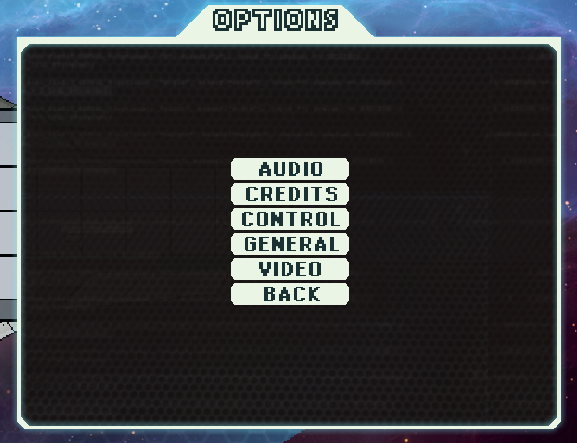
\includegraphics[width=0.5\linewidth]{images/options.png}
\end{figure}
Im Hauptmenü am Anfang des Spieles werden die Optionen aufgerufen. \\
Im Audio Unterpunkt wird erwartet, dass durch Klicken auf Mute die Musik nicht weiter abgespielt wird. Der Test war erfolgreich. \\
Durch erneutes Drücken auf den selben Knopf soll die Musik wieder abgespielt werden. Der Test war erfolgreich. \\
Durch Drücken auf Lower Volume (während die Musik läuft) sollte die Musik leiser werden. Der Test war erfolgreich. \\
Durch Drücken auf Raise Volume (während die Musik läuft) sollte die Musik lauter werden. Der Test war erfolgreich. \\
Im Video Unterpunkt wird erwartet, dass durch Klicken auf Fullscreen vom Fenster Mode zum Fullscreen Mode gewechselt wird.  Der Test war erfolgreich. \\
Durch erneutes Drücken sollte diese Änderung rückgängig gemacht werden.  Der Test war erfolgreich. \\
Diese Tests werden im GamePlay Optionen Menü erfolgreich wiederholt. \\



%%% KAMPF
\subsection{Tests zum Kampf}
Ab diesem Punkt wird davon ausgegangen, dass das Spiel gestartet ist und sich der Spieler auf einem Combat/Miniboss Planeten mit einem Gegner befindet. \\
\begin{figure}[h!]
\centering

\includegraphics[width=0.5\linewidth]{images/battle.png}
\end{figure}
\subsubsection{Next Round} 
Es wird erwartet, dass nach dem Drücken auf Next Round die eigenen Runde beendet, die eigenen Aktionen und danach die Aktionen des Gegners ausgeführt werden. Die Views updaten sich nur nach dem Drücken auf Next Round.  Der Test war erfolgreich. \\
\subsubsection{Crew bewegen}
Es wird auf einen Crew Knopf an der ganz linken Seite gedrückt, und ein Raum im eigenen Schiff ausgewählt. Nach drücken auf Next Round soll die Crew im richtigen Raum stehen. Der Test war erfolgreich. \\
Es wird auf einen Crew Knopf an der ganz linken Seite gedrückt. Danach soll auf keinen anderen Knopf außer den Raumknöpfen gedrückt werden können. Durch Drücken auf Space wird diese Änderung zurückgenommen.  Der Test war erfolgreich. \\
Es wird auf einen Crew Knopf an der ganz linken Seite gedrückt, und danach auf einen Knopf im anderen Schiff. Es soll nichts passieren. Der Test war erfolgreich. \\
\subsubsection{Waffe abschießen}
Es wird auf einen Waffen Knopf in der Box unten gedrückt. Danach wird ein Raum im feindlichen Schiff gedrückt. Es erscheint ein Target auf dem ausgewählten Tile, und nach drücken auf den Next Round Button sollte auf diesen Raum gefeuert werden. Mit den Ausgaben auf der Konsole kann dies bestätigt werden. Die Targets werden entfernt.  Der Test war erfolgreich. \\
\subsubsection{Fliehen}
Es wird nach vollständingem Aufladen des FTL Charge die Map geöffnet und ein Planet ausgewählt. Das Fliehen sollte mit einer gewissen Chance möglich sein. Das wird dadurch überprüft, diese Aktionen wiederholt durchzuführen. Der Test war erfolgreich. \\
\subsubsection{Gewinnen}
Es wird der Gegner mit Waffen angegeriffen, bis die Lebensenergie leer ist und der Gegner besiegt wurde. Der Gegner sollte verschwinden, und der normale Spielbetrieb sollte wieder aufgenommen werden.  Der Test war erfolgreich. \\
\subsubsection{Verlieren}
Man lässt sich durch wiederholtes Drücken auf Next Round ohne ausführen von Aktionen vom Gegner besiegen. Es sollte ein Game Over Screen erscheinen, und das Zurückkehren zum Hauptmenü möglich sein, ohne dass das Spiel crasht.  Der Test war erfolgreich. \\
\subsubsection{Normale Funktionen} 
Es soll weiterhin möglich sein, das Inventar zu öffnen und Waffen zu equippen/unequippen (sie Tests zum Inventar). Die Waffen sollten dann direkt für die Kampfrunde verfügbar sein. Der Test war erfolgreich. \\
Es soll weiterhin möglich sein, Energie in die Systeme zu machen und Energie zu entfernen (sie Tests zur Energieverwaltung), die dann auch so in der aktuellen Kampfunde zur Verfügung stehen. Der Test war erfolgreich. \\



%%% SHOP
\subsection{Tests zum Shop}
Ab diesem Punkt wird davon ausgegangen, dass das Spiel gestartet ist und sich der Spieler auf einem Shop Planeten befindet. \\
\begin{figure}[h!]
\centering
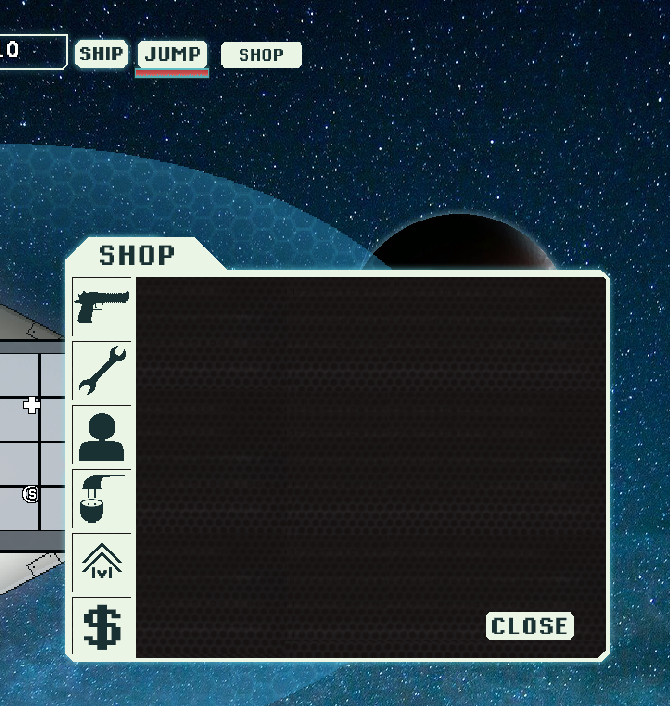
\includegraphics[width=0.5\linewidth]{images/shop.png}
\end{figure}
\subsubsection{Waffe kaufen}
Es wird auf den Waffen Knopf an der linken Seite des Shops (ganz oben) gedrückt. Es sollten Waffen angezeigt werden. Wenn auf eine Waffe gedrückt wird, die man sich leisten kann, sollte die Waffe aus dem Shop entfernt werden, und in das eigene Inventar hinzugefügt werden. Ebenfalls sollte die Geldanzeige aktualisiert werden.  Der Test war erfolgreich. \\
\subsubsection{System installieren}
Es wird auf den System Upgrade Knopf auf der linken Seite des Shops gedrückt. Es sollten die Systeme, die das Schiff haben kann, aber noch nicht unlocked hat, angezeigt werden (wie Schilde in Stealth). Wenn man es sich leisten kann, und auf den Knopf des Systems drückt, sollte es möglich werden, Energie in das System zu machen.  Der Test war erfolgreich. \\ 
\subsubsection{System upgraden}
\subsubsection{Crew kaufen}
Es wird auf den Crew Knopf auf der linken Seite gedrückt. Dort sollen alle Crew Mitglieder, die der Trader im Angebot hat, angezeigt werden. Die Crew Mitglieder sollen die gleichen Texturen haben wie die, die schon im Schiff sind. Wenn man sich ein Crew Mitglied leisten kann und auf das Crew Mitglied drückt, sollte es aus dem Shop entfernt, und der eigenen Anzeige hinzugefügt werden. Das Geld sollte angezeigt werden.  Der Test war erfolgreich. \\
\subsubsection{Waffe verkaufen}
Es wird auf den untersten Knopf auf der linken Seite gedrückt. Dort sollen alle Waffen, die man im Inventar hat, angezeigt werden. Wenn man auf eine Waffe drückt, sollte sie aus dem eigenen Inventar verschwinden, und der Preis sollte der eigenen Geldanzeige hinzugefügt werden.  Der Test war erfolgreich. \\
\subsubsection{Ressourcen kaufen}
Es wird auf den Ressourcen Knopf auf der linken Seite gedrückt. Dort sollten Hp, Missiles, und Fuel angezeigt werden. Wenn man genug Geld hat und auf den Missile oder Fuel Knopf drückt, sollte der Preis für einen abgezogen, und eine Ressource zu der passenden Anzeige hinzugefügt werden.  Der Test war erfolgreich. \\
Wenn man auf den Hp Knopf drückt, wird die komplette Anzahl der Anzeige hinzugefügt, und der Preis von der Geldanzeige abgezogen werden.  Der Test war erfolgreich. \\



%%% ENERGIEVERWALTUNG
\subsection{Tests zur Energieverwaltung}
Für das Energiemanagment werden in der unteren linken Ecke die allgemeine, unverteilte Energie des Schiffes sowie die Systeme mit Button und ihren Energiebalken angezeigt. \\
\begin{figure}[h!]
\centering
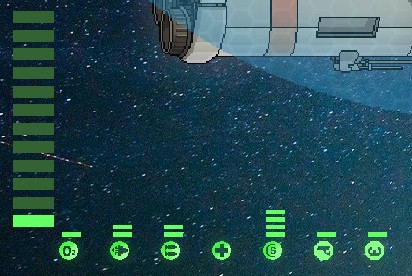
\includegraphics[width=0.5\linewidth]{images/energy1.png}
\end{figure}
\subsubsection{Energie hinzufügen}
Es wird auf den Knopf des Schild Systems gedrückt. Dadurch werden zwei Balken mehr angezeigt, und auf der linken Seite zwei weniger. Der Test war erfolgreich. \\
Für andere Systeme, wie die Engine, soll nur ein Balken hinzugefügt (und auf der linken Seite abgezogen) werden. Der Test war erfolgreich. \\
Desweiteren wird getestet, ob ein System, das vorher disabled war, enabled werden kann, indem Energie hinzugefügt wird. Dies wird an dem Beispiel des Medbays gemacht. Der Medbay wird daraufhin im Schiff normal angezeigt und hat einen Balken Energie. Der Test war erfolgreich. \\
In das Cockpit und die Cameras darf keine Energie manuell gesteckt werden können. Deswegen wird getestet, ob durch Drücken auf die zugehörigen Knöpfe Energiebalken hinzugefügt werden. Die Tests waren erfolgreich. \\
\subsubsection{Energie entfernen}
Es wird auf den Knopf für die Engine gedrückt, während zwei Balken Energie drin sind. Dadurch wird ein Balken abgezogen und an der linken Seite hinzugefügt. Der Test war erfolgreich. \\
Es wird auf den Knopf eines Systems, das keine Energie hat, gedrückt. Dadurch passiert nichts. Der Test war erfolgreich. \\
Es wird auf den Knopf eines Systems mit einem Balken Energie gedrückt. Dadurch wird der Balken abgezogen, links hinzugefügt, und das System im Schiff rot angezeigt. Der Test war erfolgreich. \\
Es wird auf den Knopf des Cockpits, und  den der Kamera gedrückt. Es passiert nichts. Der Test war erfolgreich.  \\



%%% INVENTAR
\subsection{Tests zum Inventar}
\begin{figure}[h!]
\centering
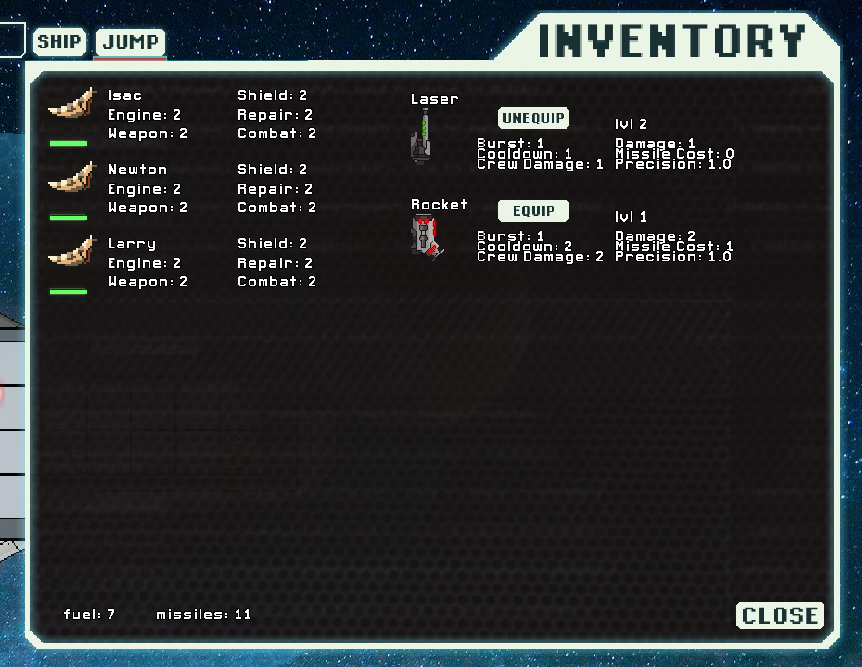
\includegraphics[width=0.5\linewidth]{images/inventory1.png}
\end{figure}
\subsubsection{Allgemein}
Durch Drücken auf den SHIP Knopf wird ein Fenster geöffnet, in dem alle Waffen und Crew Mitglieder angezeigt werden. Neben den Waffen sind die korrekten Knöpfe, falls sie equipped oder unequipped sind. Die angezeigten Werte wurden überprüft. Der Test war erfolgreich. \\
\subsubsection{Waffen equip}
Durch Drücken auf den Equip Knopf neben einer nicht equippten Waffe wird diese unten zu den equippten Waffen hinzugefügt, und der Knopf ändert sich. Der Test war erfolgreich. \\
Es wird versucht, mehr als vier Waffen zu equippen. Es passiert nichts. Der Test war erfolgreich. \\
\subsubsection{Waffen unequip}
Durch Drücken auf den Unequip Knopf neben einer Waffe wird sie unten von den equippten Waffen entfernt. Der Knopf aktualisiert sich. Der Test war erfolgreich. \\



%%% REWARDS UND PLANET EVENTS
\subsection{Tests zu Rewards und Planet Events}
\subsubsection{Planet Event Anzeige}
\begin{figure}[h!]
\centering
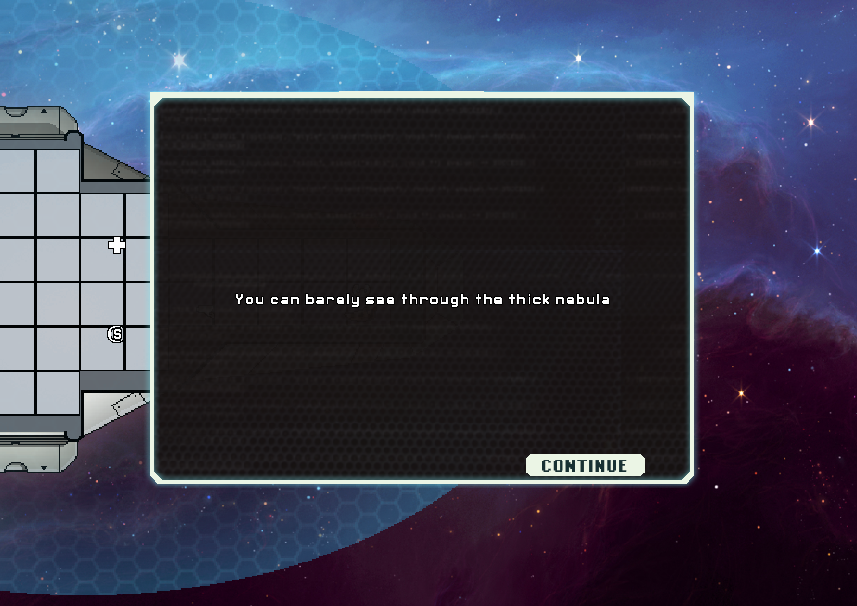
\includegraphics[width=0.5\linewidth]{images/event.png}
\end{figure}
Es werden Planeten angeflogen (Tests zum Fliegen siehe unten). Es wird für jeden Planeten ein Dialogfenster angezeigt. Der Hintergrund wird passend verändert. Der Test war erfolgreich. \\
Das Dialogfenster stimmt mit dem Event überein, welches von den Logs des Services angegeben wird. Der Test war erfolgreich. \\
Es wird ein Kampfplanet angeflogen, der Gegner besiegt, von dem Planeten weggeflogen, und wieder zum Planeten zurückgeflogen. Der Test updatet sich, um nicht wieder zu behaupten, dass ein Kampf stattfinden würde. Der Test war erfolgreich. \\
Für das Planet Event Kampf wird der Gegner angezeigt. Der Test war erfolgreich. \\
Für das Planet Event Shop wird danach ein Open Shop Button angezeigt. Der Test war erfolgreich. \\
\subsubsection{Rewards}
\begin{figure}[h!]
\centering
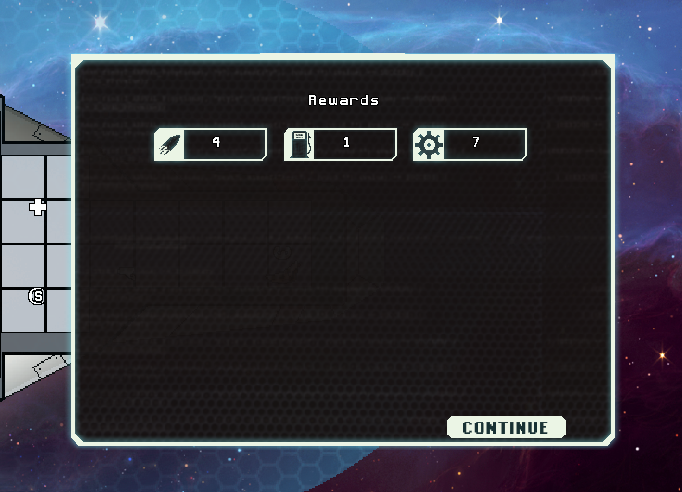
\includegraphics[width=0.5\linewidth]{images/rewards.png}
\end{figure}
Es werden Planeten angeflogen. Für die Planeten werden teilweise Reward Pages angezeigt. Es werden nur dann Reward Pages angezeigt, wenn auch tatsächlich Rewards vorhanden sind. Der Test war erfolgreich. \\
Wenn ein Reward angezeigt wird, wird erwartet, dass dieser auch hinzugefügt wird (Crew an der linken Seite, Waffe in das Inventar, Ressourcen zu den passenden Ressourcen Anzeigen). Der Test war erfolgreich. \\



%%% REISEN
\subsection{Tests zum Karte}
\begin{figure}[h!]
\centering
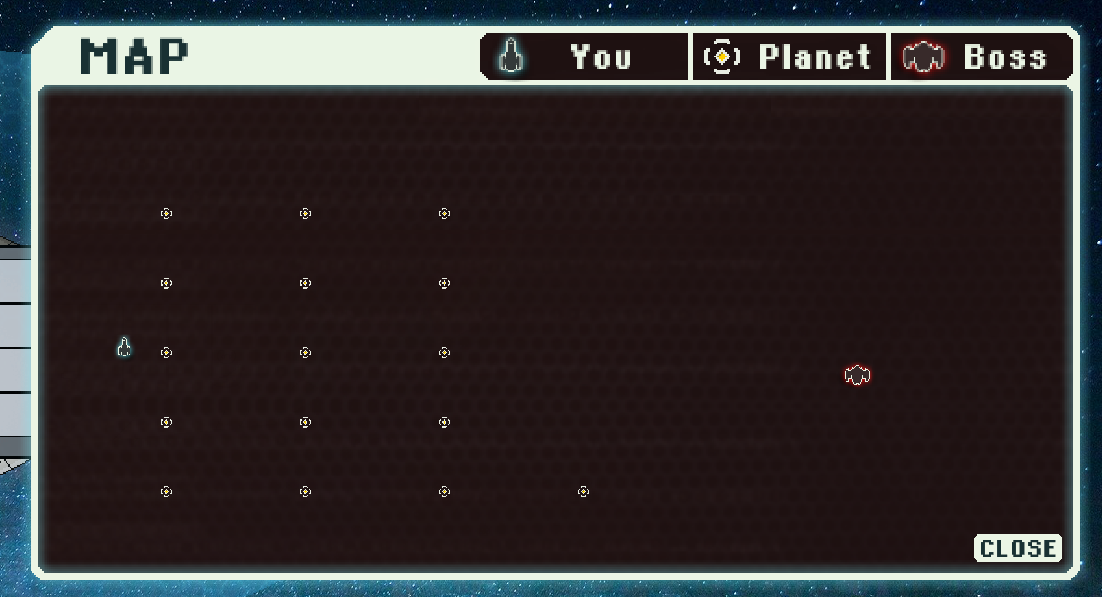
\includegraphics[width=0.5\linewidth]{images/map.png}
\end{figure}
\subsubsection{Anzeigen}
Es wird auf den Jump Button gedrückt, woraufhin die Karte mit allen Planeten, einer Kennzeichnung für den aktuellen Planeten und den Bossplaneten angezeigt werden sollte.  Der Test war erfolgreich. \\
\subsubsection{Fliegen}
Nach Drücken auf einen Planeten, der angereist werden kann (nur einen entfernt), sollte die Karte geschlossen werden und der neue Planet mit den korrekten Änderungen (Hintergrund, Events (siehe oben)) angezeigt werden. Es sollte Treibstoff entfernt werden.  Der Test war erfolgreich. \\
Nach Drücken auf einen Planeten, der nicht angereist werden kann, sollte nichts passieren.  Der Test war erfolgreich. \\

%%%%%%%%%%%%%%%%%%%%%%%%%%%	AUTOMATISIERTE
\section{Automatisierte Funktionstest}
%%% EINFÜHRUNG
\subsection{Einführung}
Projektklassen wurden unabhängig getestet. Das für die Tests verwendete Framework war Junit, Version 5. \\
Die Tests sind im Unterordner galaxytrucker/core/src/com/galaxytrucker/galaxytruckerreloaded/Test zu finden. Die Testklassen für ein Modul des Projekts finden sich im passend benannten Unterordner. \\
%%% VORGEHENSWEISE
\subsection{Vorgehensweise}
Es wurden für die Service, sowie die DAO Klassen JUNIT Tests geschrieben. \\
Die Tests für die DAOS fallen zum Teil nominell durch, da die erwarteten Exceptions, die auch geworfen werden, nicht als erwartet erkannt werden. Hierbei handelt es sich im Methoden zum löschen und updaten nicht existenter Daten. In diesen Fällen ist aber über das Nicht-Bestehen der Tests hinwegzusehen, da sie nur deshalb als nicht bestanden gelten, weil genau die Exceptions geworfen werden, die auch erwartet werden. \\

\end{document}